% id: 68-17
% book: 100발100중 3-2 중간 · 01 3-2 중간(삼각비·삼각비의 활용·원과 직선·원주각·부록)
% section: 실전 문제 1회
% figure: crop:fig-68-17.png
% answer: ⑤
% answer_source: 답지(빠른정답)
% variant_level: 0 (원본 전사)
% 이 파일은 build.mjs 가 items.json 에서 만든다. 고칠 때는 items.json 을 고친다.
\smash{\raisebox{1.5mm}{\dmkichul{100발100중 3-2 중간 68쪽 17번}}}
\noindent\begin{minipage}[t]{0.58\linewidth}\vspace{0pt}\raggedright 그림과 같이 원~$\pt{O}$가 직사각형~$\pt{ABCD}$의 세 변과 접하고 $\seg{CE}$는 원~$\pt{O}$의 접선이다. $\seg{AB}=5\mkern3mu \mathrm{cm}$, $\seg{BC}=8\mkern3mu \mathrm{cm}$일 때, $\seg{CE}$의 길이는?\end{minipage}\hfill\begin{minipage}[t]{0.4\linewidth}\vspace{0pt}\centering 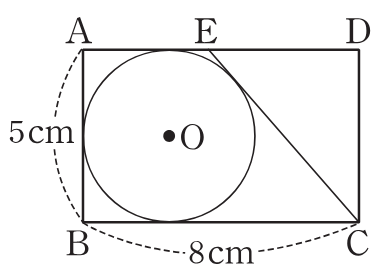
\includegraphics[width=91.1pt]{figures/fig-68-17.png}\end{minipage}\par
\begin{choices32}{\rule[-3ex]{0pt}{8ex}$\dfrac{73}{22}\mkern3mu \mathrm{cm}$}{\rule[-3ex]{0pt}{8ex}$\dfrac{83}{22}\mkern3mu \mathrm{cm}$}{\rule[-3ex]{0pt}{8ex}$\dfrac{48}{11}\mkern3mu \mathrm{cm}$}{\rule[-3ex]{0pt}{8ex}$\dfrac{68}{11}\mkern3mu \mathrm{cm}$}{\rule[-3ex]{0pt}{8ex}$\dfrac{73}{11}\mkern3mu \mathrm{cm}$}\end{choices32}
